\textbf{Глава 3} посвящена обнаруженному в работе механизму поддержания продольных вихрей. Сперва механизм дается на примере решения, имеющего вид бегущей волны. Это решение периодично вдоль потока и стационарно в сопутствующей системе отсчета. Простота пространственно-временного поведения решения позволяет на его примере более строго показать ряд закономерностей движения, обеспечивающие работу механизма. Это решение является предельным состоянием решения, эволюционирующего на сепаратрисе, найденного, в отличии от модельного порыва, в непротяженной расчетной области. В \textbf{разделе 3.1} показано, что оно повторяет особенности бегущей волны, наблюдаемой в модельном порыве, и воспроизводит общий с модельным порывом механизм поддержания колебаний. В \textbf{разделах 3.2} и \textbf{3.3} описаны механизмы поддержания продольных вихрей и пульсаций продольной завихренности на примере решения в виде бегущей волны.

В \textbf{разделе 3.4} проводится обобщение механизма поддержания продольных вихрей на модельный порыв. 
Прояснить процесс формирования продольных вихрей позволяет анализ уравнения, описывающего эволюцию средней продольной завихренности, имеющего вид
\begin{multline}\label{OX_eq}
\pd{\Omega_x}{t} + (V_x - c_f)\pd{\Omega_x}{x} + V_r \pd{\Omega_x}{r} + \frac{V_\theta}{r} \pd{\Omega_x}{\theta} - \nu\nabla^2\Omega_x= \Omega_x \pd{V_x}{x} + \Omega_r \pd{V_x}{r} + \\ + \frac{\Omega_\theta}{r} \pd{V_x}{\theta}
 - \overline{v'_x \pd{\omega'_x}{x}}^t - \overline{v'_r \pd{\omega'_x}{r}}^t - \overline{\frac{v'_\theta}{r} \pd{\omega'_x}{\theta}}^t
 + \overline{\omega'_x \pd{v'_x}{x}}^t + \overline{\omega'_r \pd{v'_x}{r}}^t + \overline{\frac{\omega'_\theta}{r} \pd{v'_x}{\theta}}^t.
\end{multline}
где $\Om = (\Omega_x, \Omega_r, \Omega_\theta)$ и $\om' = (\omega'_x, \omega'_r, \omega'_\theta)$ --- средняя и пульсационная составляющие вектора завихренности $\om = \rot \v$, $c_f$ --- скорость перемещения системы отсчета. В левой части уравнения \eqref{OX_eq} собраны конвективные и вязкие слагаемые, в правой --- источниковые, описывающие сжатие, растяжение и поворот существующих вихревых нитей и порождение средней завихренности пульсационным движением. При отсутствии пульсаций продольная завихренность постепенно исчезает под действием вязкости. В рассматриваемом течении система находится в равновесии и средняя продольная завихренность во времени не меняется. Вязкие диссипация и диффузия компенсируются генерацией завихренности членами в правой части.

Для выявления определяющих механизмов генерации средней продольной завихренности удобнее рассматривать уравнение эволюции квадрата $\Omega_x$, получающееся домножением всех членов \eqref{OX_eq} на $2\Omega_x$. Положительный или отрицательный знак у полученных таким образом выражений в правой части уравнения показывает соответственно положительный или отрицательный вклад этого члена в изменение $\Omega^2_x$, а следовательно, и в интенсивность поперечного движения. Распределение $\Omega^2_x$ по сечению трубы представлено на рисунке \ref{OXgen_pic}(a). В большей части сечения трубы средняя продольная завихренность близка к нулю. Область концентрации $\Omega_x$ расположена между полосами повышенной и пониженной скорости вблизи области максимальной амплитуды пульсаций.

При анализе уравнения \eqref{OX_eq} обнаружено, что два слагаемых в правой части, а именно
\begin{equation}\label{OXgen_terms}
- \overline{v'_x \frac{\d \omega'_x}{\d x}}^t + \overline{ \omega'_x \frac{\d v'_x}{\d x} }^t
\end{equation}
вносят определяющий вклад в производство средней продольной завихренности. Соответствующее сумме \eqref{OXgen_terms} распределение в уравнении для $\Omega^2_x$ представлено на рисунке \ref{OXgen_pic}(б), а вклад остальных слагаемых правой части \eqref{OX_eq} показан на рисунке \ref{OXgen_pic}(в). Распределение генерации $\Omega^2_x$ выделенными в \eqref{OXgen_terms} членами практически совпадает по форме с распределением $\Omega^2_x$, тогда как вклад остальных членов не имеет выраженного распределения и более чем на порядок уступает по суммарному вкладу в генерацию $\Omega^2_x$. Таким образом, нет сомнения в том, что стационарные продольные вихри возникают в основном за счет действия выделенной в \eqref{OXgen_terms} пары слагаемых.

\begin{figure}
\center{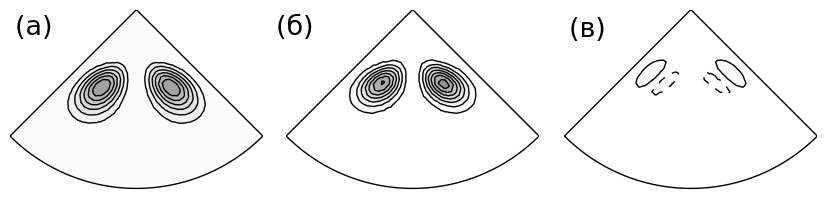
\includegraphics[width=1\linewidth]{autoref_OXgen.png}}
\caption{Механизм генерации продольных вихрей}
\label{OXgen_pic}
\end{figure}

Каждое из двух слагаемых в \eqref{OXgen_terms} дает примерно половину общего вклада в производство средней продольной завихренности. Это значит, в частности, что колебания $\partial v'_x / \partial x$ и $\omega'_x$ положительно коррелированы в области концентрации положительной $\Omega_x$ и отрицательно коррелированы в области концентрации отрицательной $\Omega_x$. То же относится и к колебаниям $-v'_x$ и $\partial \omega'_x / \partial x$. Расчет соответствующих коэффициентов корреляции показывает, что они близки к $\pm1$ в соответствующих областях. Объяснить существование такой связи позволяет механизм формирования пульсаций продольной завихренности, описанный в \textbf{разделе 3.3}. Обратимся к уравнению эволюции $\omega'_x$:
\begin{multline}\label{ox1_eq}
\pd{\omega'_x}{t} + (V_x - c_\mathrm{tw})\pd{\omega'_x}{x} + V_r \pd{\omega_x'}{r} + \frac{V_\theta}{r} \pd{\omega'_x}{\theta} 
- \nu\nabla^2\omega'_x = - v'_x \pd{\Omega_x}{x} - v'_r \pd{\Omega_x}{r} - \\ - \frac{v'_\theta}{r} \pd{\Omega_x}{\theta} 
+ \Omega_x \pd{v'_x}{x} + \Omega_r \pd{v'_x}{r} + \frac{\Omega_\theta}{r} \pd{v'_x}{\theta}
+ \omega'_x \pd{V_x}{x} + \omega'_r \pd{V_x}{r} + \frac{\omega'_\theta}{r} \pd{V_x}{\theta} - \\ 
- v'_x \pd{\omega'_x}{x} - v'_r \pd{\omega'_x}{r} - \frac{v'_\theta}{r} \pd{\omega'_x}{\theta} 
+ \omega'_x \pd{v'_x}{x} + \omega'_r \pd{v'_x}{r} + \frac{\omega'_\theta}{r} \pd{v'_x}{\theta} + \\
+ \overline{v'_x \pd{\omega'_x}{x}}^t + \overline{v'_r \pd{\omega'_x}{r}}^t + \overline{\frac{v'_\theta}{r} \pd{\omega'_x}{\theta}}^t
- \overline{\omega'_x \pd{v'_x}{x}}^t - \overline{\omega'_r \pd{v'_x}{r}}^t - \overline{\frac{\omega'_\theta}{r} \pd{v'_x}{\theta}}^t.
\end{multline}
На практике, удобнее работать с уравнением баланса среднего квадрата пульсаций продольной завихренности $\overline{\omega'_x\omega'_x}^t$, получающимся умножением \eqref{ox1_eq} на $2\omega'_x$ и последующим осреднением по времени. Слагаемые в этом уравнении не зависят от времени, сумма слагаемых в правой части балансируется вязким членом в левой части. Как и в предыдущем случае, среди всех слагаемых правой части удается выделить существенные, ответственные за возникновение пульсаций $\omega'_x$.

\begin{figure}
\center{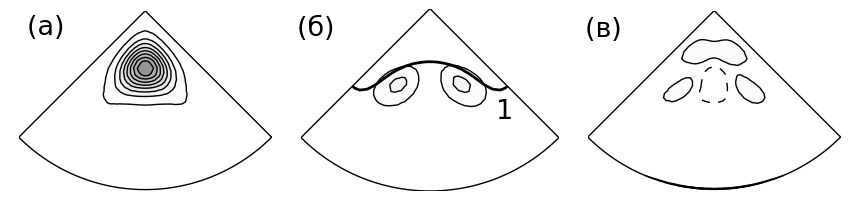
\includegraphics[width=1\linewidth]{autoref_ox1gen.png}}
\caption{Механизм генерации пульсаций продольной завихренности}
\label{ox1gen_pic}
\end{figure}

Обнаружено, что за генерацию пульсаций $\omega'_x$ в различных областях течения отвечают два разных механизма. Первый связан с поворотом нормальных к стенке вихрей на фоне нормального к стенке градиента скорости. За этот механизм отвечают два слагаемых в правой части \eqref{ox1_eq}:
\begin{equation}\label{ox1gen_add_terms}
\frac{\d \omega'_x}{\d t} = \omega'_r \frac {\d V_x}{\d r} + \frac{\Omega_\theta}{r} \frac{\d v'_x}{\d \theta} + ...
\end{equation}
Вклад слагаемых \eqref{ox1gen_add_terms} в производство  $\overline{\omega'_x\omega'_x}^t$ приведен на рисунке \ref{ox1gen_pic}(a). Они производят пульсации $\omega'_x$ существенной амплитуды в области между полосой пониженной скорости и осью трубы, но производимые ими пульсации практически не участвуют в поддержании продольных вихрей, так как не имеют необходимой для этого согласованности фаз с пульсациями $v'_x$.

Второй механизм образования пульсаций продольной завихренности $\omega'_x$ связан с перераспределением уже существующей стационарной продольной завихренности $\Omega_x$ пульсационной составляющей продольной скорости $v'_x$ (эффект сжатия/растяжения вихревых трубок). В уравнении \eqref{ox1_eq} за описываемый механизм отвечает слагаемое
\begin{equation}\label{ox1gen_main_terms}
\frac{\d \omega'_x}{\d t} = \Omega_x \frac {\d v'_x}{\d x} + ...
\end{equation}
Выделенное в \eqref{ox1gen_main_terms} слагаемое стремится произвести пульсации $\omega'_x$, пропорциональные $\d v'_x / \d x$, причем коэффициентом пропорциональности выступает средняя продольная завихренность. Соответственно, механизм включается в областях концентрации~$\Omega_x$. В области расположения положительного вихря производимые пульсации $\omega'_x$ положительно пропорциональны пульсациям $\d v'_x / \d x$, а в области расположения отрицательного вихря --- отрицательно пропорциональны. Таким образом обеспечивается максимально возможная эффективность производства средней продольной завихренности нужного знака посредством второго из слагаемых \eqref{OXgen_terms}. Пульсации $-v'_x$ и $\d \omega'_x / \d x$ отказываются также согласованы нужным образом, и первое слагаемое \eqref{OXgen_terms} оказывается равно второму.

На рисунке \ref{ox1gen_pic}(б) приведен вклад выделенного в \eqref{ox1gen_main_terms} слагаемого в производство $\overline{\omega'_x\omega'_x}^t$. Нет сомнения, что именно это слагаемое определяет форму пульсаций в области существования продольных вихрей между полосами повышенной и пониженной скорости. Суммарный вклад других слагаемых правой части \eqref{ox1_eq}, не попавших на рисунки \ref{ox1gen_pic}(а, б), изображен на рисунке \ref{ox1gen_pic}(в). Эти слагаемые не имеют существенного значения в процессе генерации $\omega'_x$, их суммарный вклад не превышает нескольких процентов.

Описанный механизм генерации пульсаций продольной завихренности проявляется в области, где фазовая скорость волны, соответствующей пульсационной составляющей течения, близка по значению к локальной продольной скорости среднего течения (см. фиг. 2, б). На удалении от точки генерации пульсаций, где фазовая скорость волны существенно отличается от средней скорости, выделенный в \eqref{ox1gen_main_terms} механизм генерации $\omega'_x$ практически не работает. Это объясняется тем, что в системе отсчета, связанной с волной, образующаяся посредством механизма \eqref{ox1gen_main_terms} $\omega'_x$ сносится вдоль трубы средним течением. При этом теряется согласованность фаз между $\d v'_x / \d x$ и $\omega'_x$, что делает ее рост невозможным.

Описанный механизм генерации пульсаций продольной завихренности объясняет необходимость учета поперечного движения при исследовании устойчивости стационарного течения. Пренебрежение связанной с поперечным движением $\Omega_x$ делает невозможным генерацию $\omega'_x$ в форме, необходимой для сохранения поперечного движения, а следовательно и всего процесса самоподдержания пульсаций.

В \textbf{разделе 3.5} приведены выводы по главе. Основные результаты главы опубликованы в работах автора диссертации \cite{MZG2017,  KMU17}. 
